\chapter{Conclusión y trabajo futuro} \label{conclusion}

En este capítulo final se muestran las conclusiones en base a los resultados mostrados. Se valorará cada uno de los algoritmos y se verán sus ventajas y desventajas. Además, se valorará la viabilidad de aplicar estos algoritmos en circuitos neuromórficos. Para concluir, se mostrará posibles lineas de investigación a seguir en un futuro. 

Para una mejor comparación, voy a mostrar los resultados de los algoritmos arquitectura por arquitectura. Seleccionaré de entre las funciones de cuantificación, la mejor para cada algoritmo.

\section{Comparación de los algoritmos}

Comenzaremos analizando los modelos bases.
\begin{figure}[H]
    \centering
    \begin{subfigure}[H]{0.475\textwidth} 
    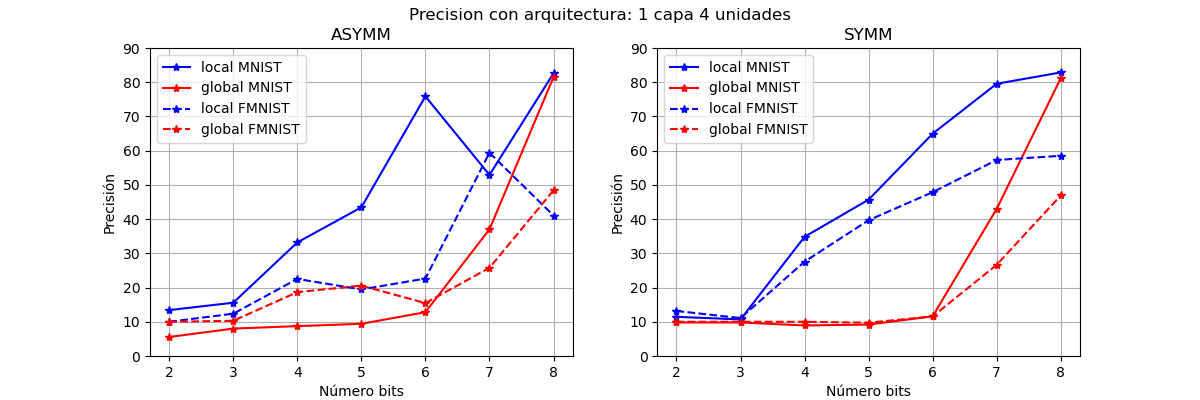
\includegraphics[width=\textwidth]{imagenes/backprop/Precision con arquitectura: 1 capa 4 unidades.png}
    \caption{Backpropagation}
    \end{subfigure}
    \begin{subfigure}[H]{0.475\textwidth}
    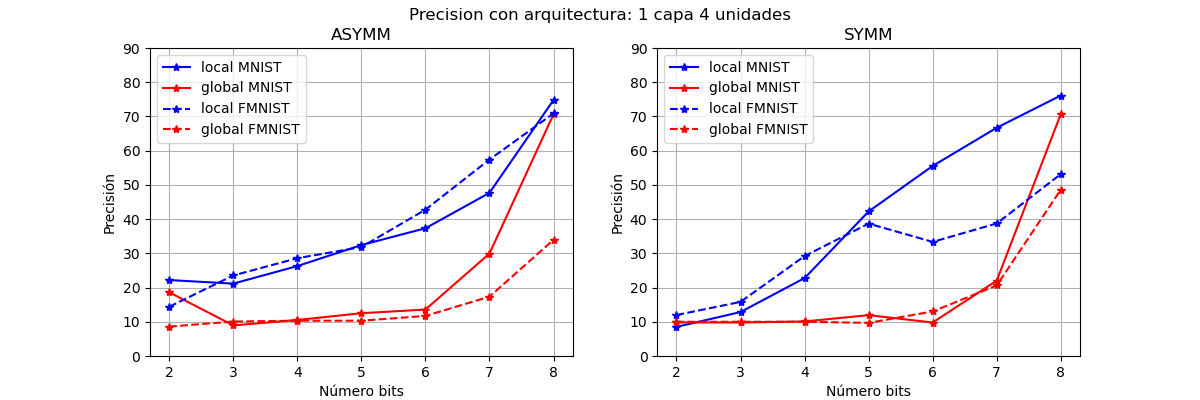
\includegraphics[width=\textwidth]{imagenes/fa/Precision con arquitectura: 1 capa 4 unidades.png}
    \caption{Feedback Alignment}
    \end{subfigure}
    \begin{subfigure}[H]{0.475\textwidth}
    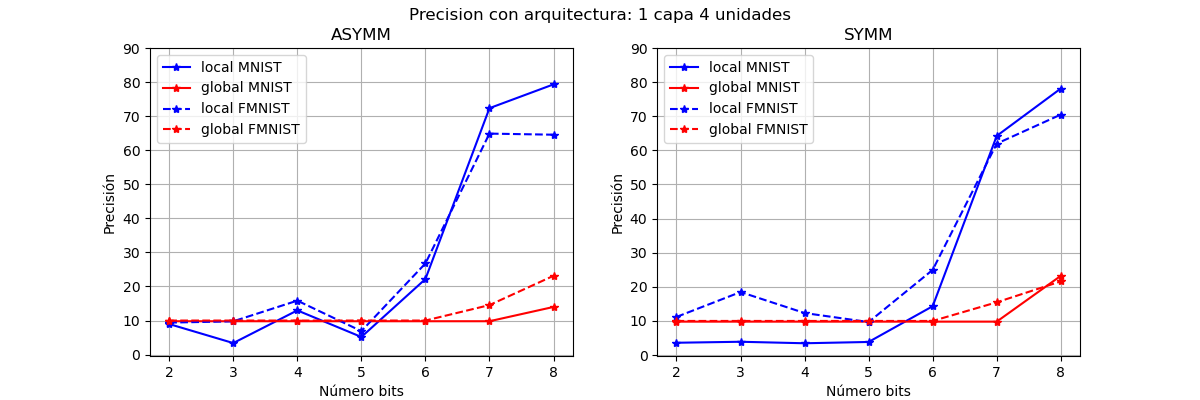
\includegraphics[width=\textwidth]{imagenes/HSIC/Precision con arquitectura: 1 capa 4 unidades.png}
    \caption{HSIC}
    \end{subfigure}
    \begin{subfigure}[H]{0.475\textwidth}
    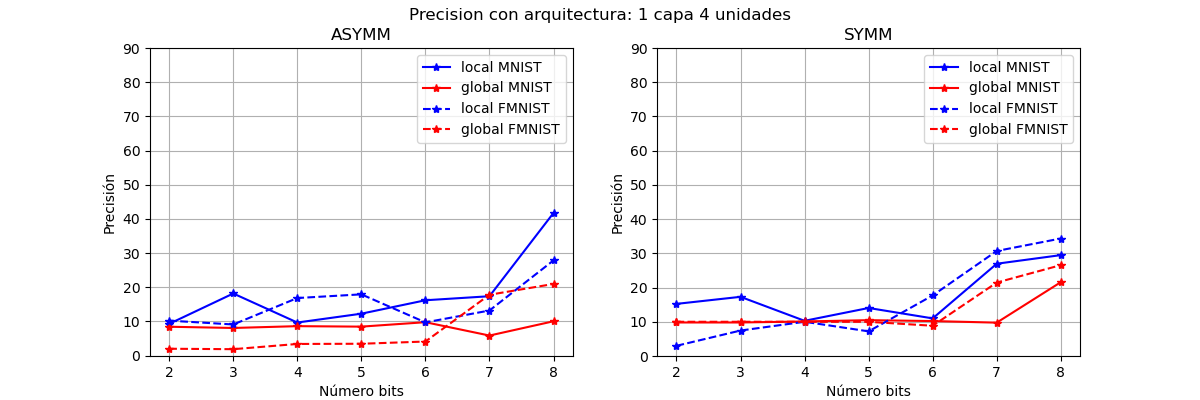
\includegraphics[width=\textwidth]{imagenes/dni/Precision con arquitectura: 1 capa 4 unidades.png}
    \caption{Synthetic Gradient}
    \end{subfigure}
    \caption{Comparación modelos bases}
    %\label{fig:my_label}
\end{figure}

Comparando las 4 gráficas, el modelo que peor desempeño tiene es el de Synthetic gradient. Como se comentó en su respectivo Apartado \ref{synthetic gradient}, este algoritmo no puede ser aplicado con cuantificación (en las arquitecturas estudiadas). Como en ninguna de las arquitecturas estudiadas ha conseguido resultados viables, no se va a usar en las siguientes comparaciones.  

Fijémonos ahora en los 3 algoritmos restantes. Las gráficas que más se asemejan son la de Backpropagation y Feedback Alignment. Ambos algoritmos consiguen precisiones muy parecidas, sin embargo, el backpropagation obtiene mejores resultados en FMNIST cuando usa la cuantificación local. Además, en los modelos cuantificados globalmente con 7 y 8 bits, Backpropagtation es ligeramente superior. Si observamos ahora HSIC, vemos que a nivel global es inferior los dos algoritmos mencionados, y a nivel local es inferior hasta los 8 bits. Cuando se alcanza el máximo número de bits con cuantificación local, HSIC es el algoritmo que mejores precisiones alcanza, 70\% en FMNIST y 80\% en MNIST. Por lo tanto, con arquitecturas pequeñas y por debajo de los 8 bits, el algoritmo que mejores resultados ofrece es el clásico Backpropagation. Sin embargo, llegado a los 8 bits, el que mejor resultados alcanza es HSIC.

Pasemos ahora a las arquitecturas con 6 capas ocultas. 

\begin{figure}[H]
    \centering
    \begin{subfigure}[H]{0.475\textwidth}
    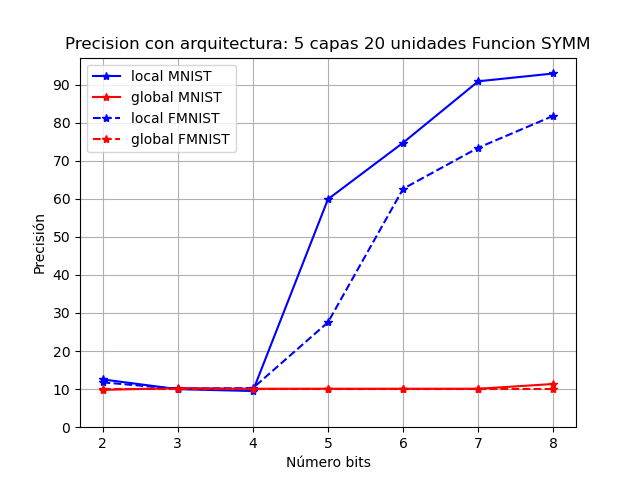
\includegraphics[width=\textwidth]{imagenes/backprop/Precision con arquitectura: 5 capas 20 unidades Funcion SYMM.png}
    \caption{Backpropagation}
    \end{subfigure}
    \begin{subfigure}[H]{0.475\textwidth}
    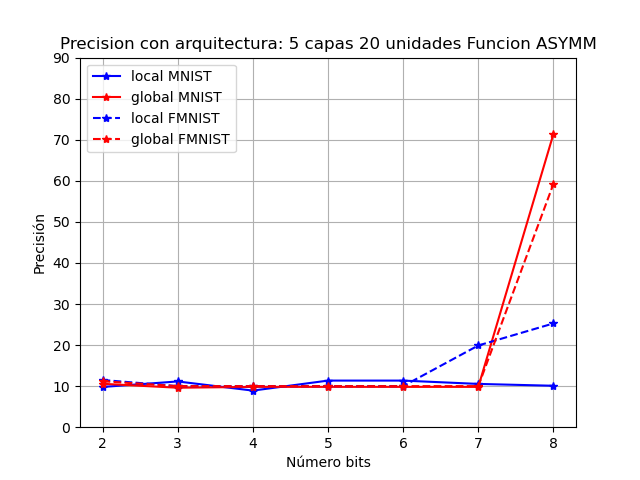
\includegraphics[width=\textwidth]{imagenes/fa/Precision con arquitectura: 5 capas 20 unidades Funcion ASYMM.png}
    \caption{Feedback Alignment}
    \end{subfigure}
    \begin{subfigure}[H]{0.475\textwidth}
    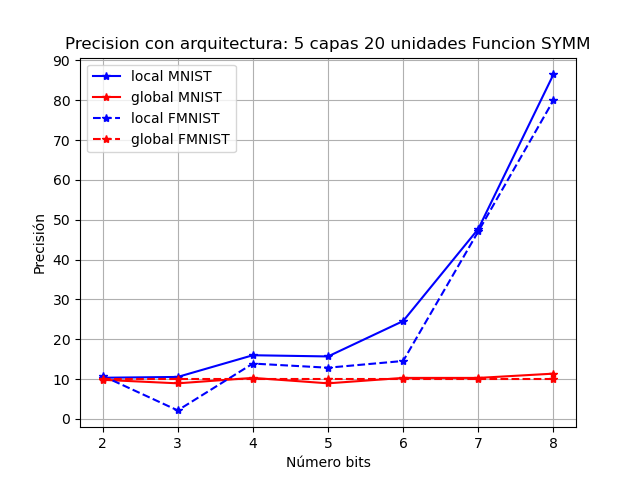
\includegraphics[width=\textwidth]{imagenes/HSIC/Precision con arquitectura: 5 capas 20 unidades Funcion SYMM.png}
    \caption{HSIC}
    \end{subfigure}
    \caption{Comparación arquitecturas: 6 capas ocultas y 20 neuronas}
\end{figure}

Con cuantificación local el mejor algoritmo es el Backpropagation. 7 bits son suficientes para conseguir precisiones elevadas, 90\% MNIST y 80\% FMNIST. Mientras que para la cuantificación a nivel global, el mejor algoritmo es el de Feedback Alignment, consiguiendo un 60\% y 70\% para FMNIST y MNIST respectivamente. Por lo tanto, para modelos profundos el mejor algoritmo es el Backpropagation.

Veamos ahora los modelos con arquitecturas anchas (50-100 neuronas) y 2 capas ocultas. 

\begin{figure}[H]
    \centering
    \begin{subfigure}[H]{0.475\textwidth}
    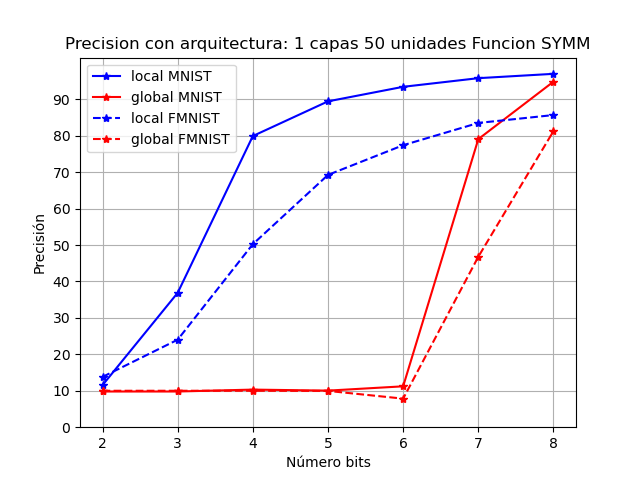
\includegraphics[width=\textwidth]{imagenes/backprop/Precision con arquitectura: 1 capas 50 unidades Funcion SYMM.png}
    \caption{Backpropagation}
    \end{subfigure}
    \begin{subfigure}[H]{0.475\textwidth}
    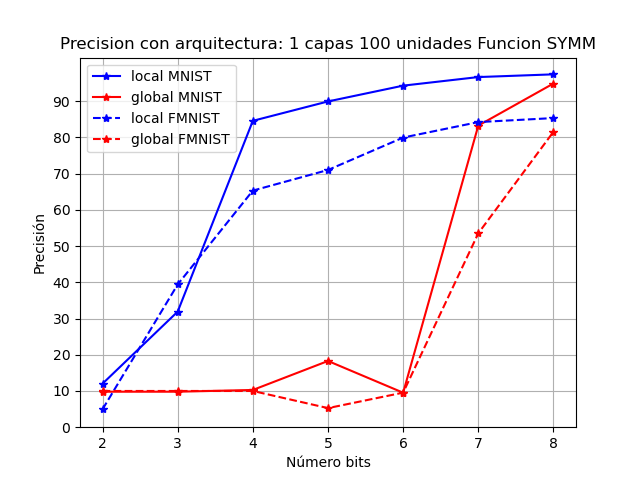
\includegraphics[width=\textwidth]{imagenes/backprop/Precision con arquitectura: 1 capas 100 unidades Funcion SYMM.png}
    \caption{Backpropagation}
    \end{subfigure}
    \begin{subfigure}[H]{0.475\textwidth}
    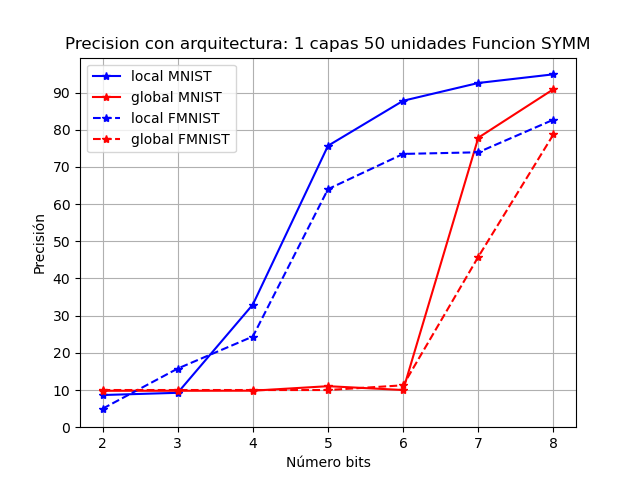
\includegraphics[width=\textwidth]{imagenes/fa/Precision con arquitectura: 1 capas 50 unidades Funcion SYMM.png}
    \caption{Feedback Alignment}
    \end{subfigure}
    \begin{subfigure}[H]{0.475\textwidth}
    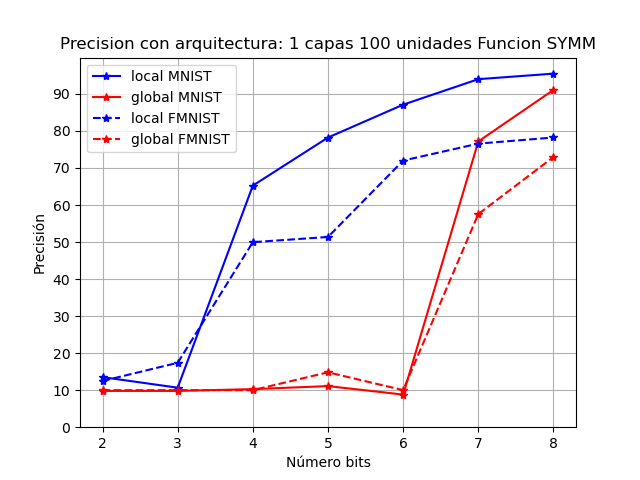
\includegraphics[width=\textwidth]{imagenes/fa/Precision con arquitectura: 1 capas 100 unidades Funcion SYMM.png}
    \caption{Feedback Alignment}
    \end{subfigure}
    \begin{subfigure}[H]{0.475\textwidth}
    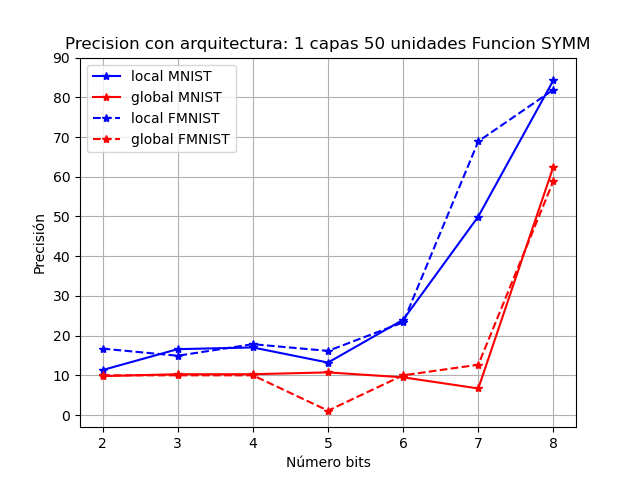
\includegraphics[width=\textwidth]{imagenes/HSIC/Precision con arquitectura: 1 capas 50 unidades Funcion SYMM.png}
    \caption{HSIC}
    \end{subfigure}
    \begin{subfigure}[H]{0.475\textwidth}
    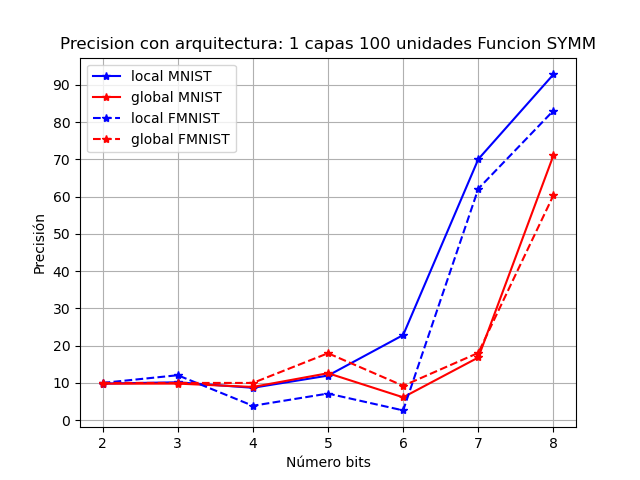
\includegraphics[width=\textwidth]{imagenes/HSIC/Precision con arquitectura: 1 capas 100 unidades Funcion SYMM.png}
    \caption{HSIC}
    \end{subfigure}
    \caption{Comparación arquitecturas: 6 capas ocultas y 20 neuronas}
\end{figure}

Con estas arquitecturas el algoritmo que mayor precisión obtiene con cuantificación local, es el Backpropagation. No solamente alcanza las precisiones máximas con 8 bits, si no que también es capaz de obtener precisiones elevadas a partir de 5 bits de precisión. FeedBack Alignmente le sigue muy de cerca en los resultados, aunque necesita mínimo 6 bits para conseguir precisiones elevadas. Mientras tanto, HSIC necesita 8 bits para poder competir con estos algoritmos. En cuanto a la cuantificación global, Backpropagation y Feedback Aligment están empatados, necesitando 8 bits para alcanzar precisiones elevadas en ambos problemas. Mientras que HSIC no consigue obtener resultados tan elevados con la cuantificación global. Además de ver que algoritmo es mejor, podemos apreciar que un aumento de la anchura de la red mejora la precisión de los modelos.

Finalmente nos queda por evaluar las arquitecturas con 3 capas ocultas y 50 y 100 neuronas.

\begin{figure}[H]
    \centering
    \begin{subfigure}[H]{0.475\textwidth}
    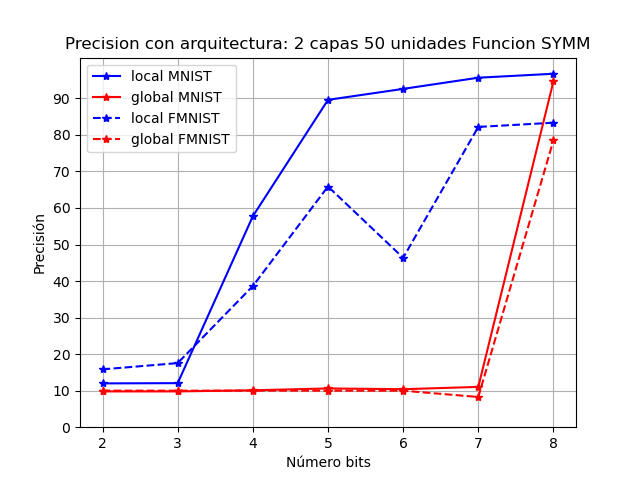
\includegraphics[width=\textwidth]{imagenes/backprop/Precision con arquitectura: 2 capas 50 unidades Funcion SYMM.png}
    \caption{Backpropagation}
    \end{subfigure}
    \begin{subfigure}[H]{0.475\textwidth}
    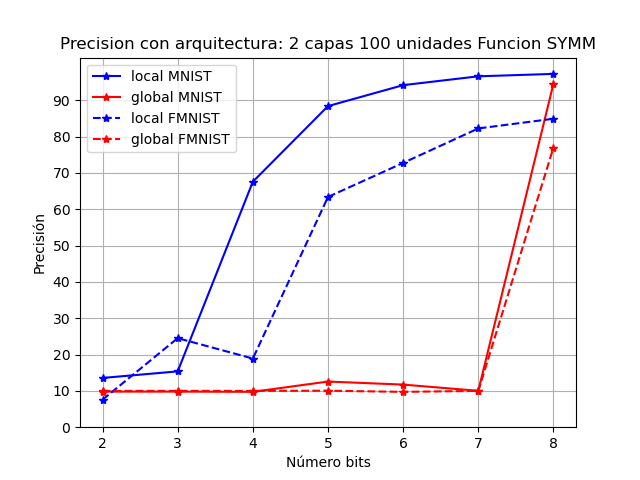
\includegraphics[width=\textwidth]{imagenes/backprop/Precision con arquitectura: 2 capas 100 unidades Funcion SYMM.png}
    \caption{Backpropagation}
    \end{subfigure}
    \begin{subfigure}[H]{0.475\textwidth}
    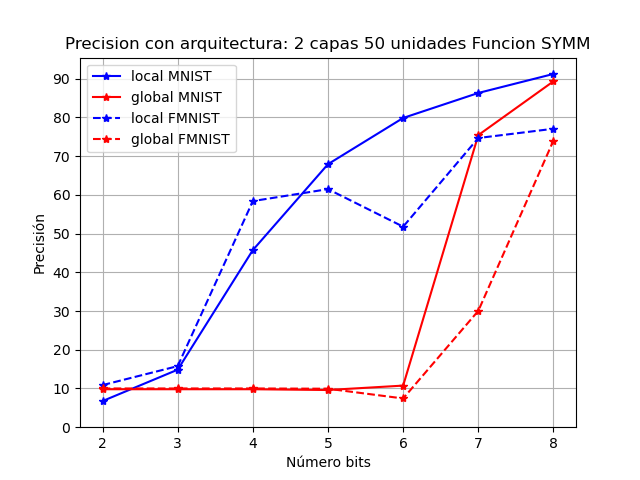
\includegraphics[width=\textwidth]{imagenes/fa/Precision con arquitectura: 2 capas 50 unidades Funcion SYMM.png}
    \caption{Feedback Alignment}
    \end{subfigure}
    \begin{subfigure}[H]{0.475\textwidth}
    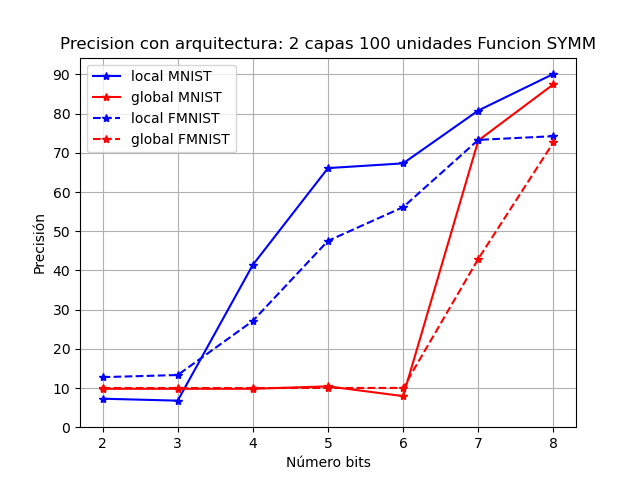
\includegraphics[width=\textwidth]{imagenes/fa/Precision con arquitectura: 2 capas 100 unidades Funcion SYMM.png}
    \caption{Feedback Alignment}
    \end{subfigure}
    \begin{subfigure}[H]{0.475\textwidth}
    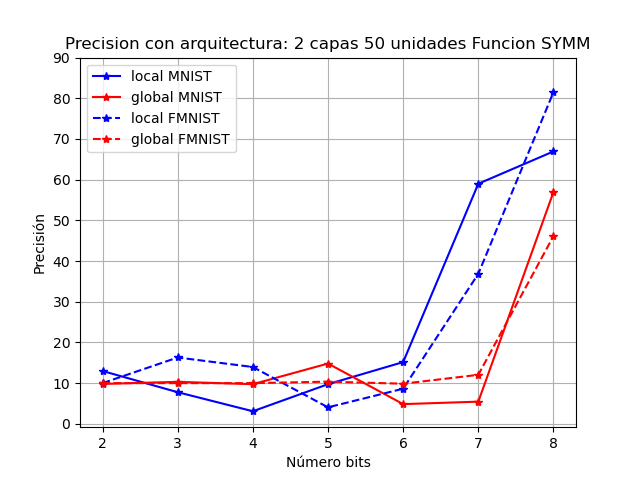
\includegraphics[width=\textwidth]{imagenes/HSIC/Precision con arquitectura: 2 capas 50 unidades Funcion SYMM.png}
    \caption{HSIC}
    \end{subfigure}
    \begin{subfigure}[H]{0.475\textwidth}
    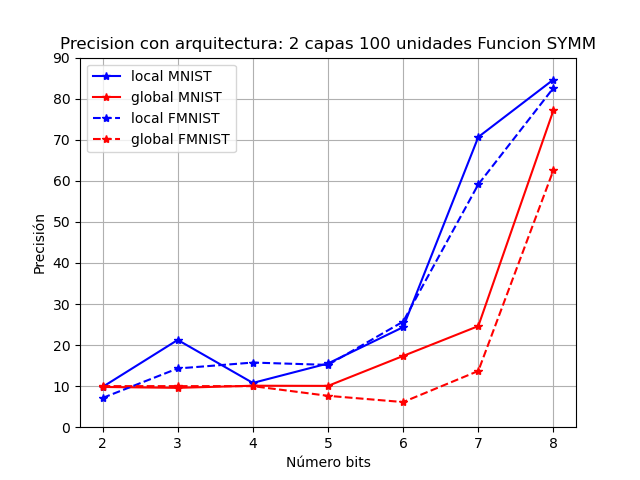
\includegraphics[width=\textwidth]{imagenes/HSIC/Precision con arquitectura: 2 capas 100 unidades Funcion SYMM.png}
    \caption{HSIC}
    \end{subfigure}
    \caption{Comparación arquitecturas: 6 capas ocultas y 20 neuronas}
\end{figure}

Las gráficas son muy similares a las de las arquitecturas de 2 capas. Se mantiene el hecho de a mayor anchura mejores resultados, y que el Backpropagation es el mejor de los 3 algoritmos. Sin embargo, en comparación con los modelos de 2 capas, las precisiones decaen ligeramente.

\section{Revisión de las hipótesis}

Expuestos los resultados de la experimentación y hechas las comparaciones entre los algoritmos, se procede a confirmar o refutar las hipótesis formuladas. HABLAR SOBRE LOS RESULTADOS SIN CUANTIFICACIÓN.

\subsection{Límite de cuantificación en torno a 6 o 7 bits}
Se ha podido apreciar en la experimentación, que los algoritmos de Backpropagation y Feedback Alignment pueden conseguir precisiones elevadas por debajo de este umbral con cuantificación local. Como se ha comentado en la experimentación, este tipo de cuantificación se ha estudiado con el fin de ver si existe una mejora cuando las redes trabajan mejor con distintos rangos de valores por capa. A la luz de los resultados esto es así, por lo tanto, a futuro se tendría que investigar algún método para hacer la estimación de dichos rangos. Por su parte, centrándonos en las cuantificaciones globales (las más fieles a la realidad), podemos ver que para conseguir precisiones elevadas se necesitan 7 u 8 bits, dependiendo del problema y la arquitectura. Por lo tanto, nuestra hipótesis inicial se cumple.

\subsection{ASYMM y SYMM ofrecen mismo rendimiento}

Con un simple vistazo a los resultados se puede apreciar que esta hipótesis queda totalmente refutada. La función ASYMM mete mucho ruido de cuantificación, llegado a los 6 bits este ruido afecta notoriamente al proceso de búsqueda, haciendo que en ciertos casos la búsqueda diverja y no encuentre óptimos. Por su parte, la función SYMM no introduce tanto ruido permitiendo a los modelos alcanzar buenos óptimos.

\subsection{Mejor algoritmo: HSIC}

Otra hipótesis que queda refutada con los resultados. Como hemos podido apreciar, alcanzado los 8 bits este modelo consigue alcanzar precisiones elevadas, sin embargo, es superado tanto por el Backpropagation como por el Feedback Alignment. Además, con menos de 7 bits, este algoritmo ya se mediante cuantificación local o global, no consigue alcanzar precisiones elevadas.

\subsection{Parámetro diferencial arquitecturas: Anchura}

Este hipótesis se puede confirmar con los resultados ofrecidos. En todos los algoritmos, cuando se ha aumentado la anchura de las redes, se han conseguido elevar notoriamente la precisión. Siendo mucho más importante la anchura que la profundidad. Además, hemos visto que aumentada la profundidad, la precisión puede llegar a decaer. En conclusión, las arquitecturas con anchura elevada permiten alcanzar precisiones más elevadas.

\section{Es viable entrenar redes neuronales en circuitos neuromórficos}

Ahora toca responder a la pregunta inicial de este proyecto. ¿Es viable entrenar redes neuronales totalmente conectada en circuitos neuromórficos? Con las arquitecturas estudiadas y los algoritmos seleccionados, la respuesta es: a día de hoy no es posible. La precisión alcanzada por los memristores es de 2 a 3 bits, y en base a los resultados, estas precisiones son muy pobres. Con estas arquitecturas y algoritmos estudiados hemos visto que se necesita mínimo una precisión de 7 u 8 bits para alcanzar precisiones elevadas. Por lo tanto, entrenar estos modelos en memristores de 3 bits no es posible.  

\section{Trabajo futuro}

El estudio realizado durante este proyecto se ha ajustado a las horas que se emplean en un TFG. Por lo tanto, aun queda un gran número de factores por estudiar, como son: 
\begin{itemize}
    \item \textbf{Tipos de redes}: convolucionales, recurrentes, transformers, etc.
    \item \textbf{Hiperparámetros}: coeficiente de aprendizaje, número de iteraciones, optimizador a usar, etc.
    \item \textbf{Algoritmos de entrenamiento}: explorar nuevos algoritmos de entrenamiento. 
\end{itemize}

Otro factor muy importante que se tendría que estudiar es el método de actualización de los pesos. Los algoritmos estudiados varían a la hora de calcular el gradiente, pero los pesos se actualizan de la misma forma: gradiente descendente. Así que estudiar una alternativa sería interesante. 